\section{基于超像素表达的面向目标提取最优分割方法}

传统的最优分割方法一般是基于图像像素进行的,而基于超像素表达的最优分割方法是基于超像素的。在对原始图像进行超像素分割之后,在超像素块的基础上,进行超像素块的合并,得到最终最优分割结果。

本部分的超像素表达使用 SLIC 算法进行。

\subsection{谱聚类方法简介}

聚类就是根据样本之间的相似度,将它们分成不同组的过程。谱聚类的思想是将样本看作图节点$V$,样本间的相似度看作带权的边$E$,这样就能得到一个无向图$G=(V,E)$,从而将聚类问题转化为图分割问题:即找到一种划分方法,使得不同组间边的权重尽可能的低(这意味着组间相似度尽可能低),组内边的权重尽可能高(这意味着组内相似度尽可能高)。


\begin{figure}[H]
\centering
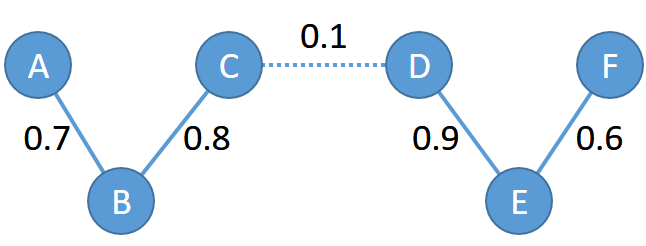
\includegraphics[width=7.5cm]{figures/谱聚类原理图.png}
\captionsetup{justification=centering}
\caption{谱聚类原理图 \\ Fig.\ref{谱聚类原理图} The Principle Diagram of the Spectral Clustering}\label{谱聚类原理图}
\end{figure}

在图\ref{谱聚类原理图}中,总共有$6$个节点,节点间连线上的数字表示两个节点间的相似度,如果现在要将这图分成两类,根据谱聚类的思想,应该去掉的边是用虚线表示的那一条边,这样就形成了两类节点。

由于本部分只使用到了非标准谱聚类算法,所以这里只介绍非标准谱聚类算法的执行步骤,谱聚类算法的步骤如下:

1. 假设输入数据的聚类数量为$k$,首先,定义数据之间相似度的度量标准,根据数据构造一个图,图的每一个节点对应一个数据点,将图中相邻的节点连接起来,数据之间的相似度用节点间边的权重来表示。把这个图用相似度矩阵的形式表示出来,记为$W$,相似度矩阵一般的计算公式为
$$
W_{ij}=\exp{(\frac{\|x_i-x_j\|^2}{2\sigma^2})}
$$

其中,$\sigma$为需要人工设定的参数,谱聚类算法的分类效果很大程度上取决于参数$\sigma$选取的合适与否;

2. 把相似度矩阵$W$中每一列的元素加起来得到$N$个数,把他们放到对角线上构成一个$N\times N$的对角矩阵,记为$D$,计算非标准化图的拉普拉斯矩阵$L=D-W$;

3. 求出$L$的前$k$个最小的特征值,以及特征值对应的特征向量$u_1,\cdots,u_k$;

4. 将这$k$个特征向量组成一个$N\times k$的矩阵$U$;

5. 将矩阵$U$的第$i$行作为行向量$(y_i)_{i=1,\cdots,n}$;

6. 对行向量$(y_i)_{i=1,\cdots,n}$使用$k$-means算法进行聚类,得到$k$个聚类$C_1,\cdots,C_k$[23]。

\begin{figure}[H]
    \centering
    \subfigure[聚类前原始数据]
    {
        \label{Fig.sub.1}
        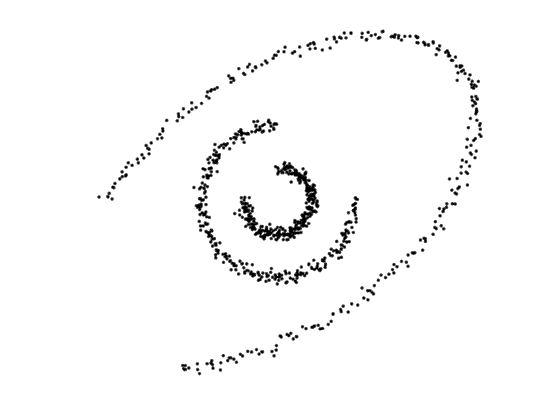
\includegraphics[width=3.8cm]{figures/聚类前原始数据.png}
    }
    \subfigure[谱聚类分类结果]
    {
        \label{Fig.sub.2}
        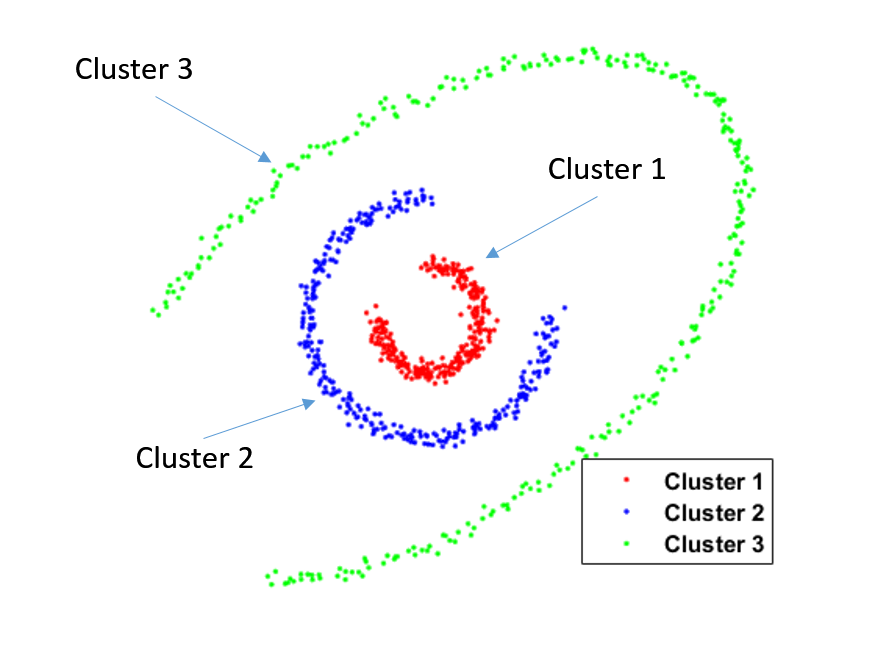
\includegraphics[width=3.8cm]{figures/谱聚类分类结果.png}
    }
    \captionsetup{justification=centering}
    \caption{谱聚类分类效果示意图 \\ Fig.\ref{谱聚类分类效果示意图} Spectral Clustering Classification Effect Diagram}
    \label{谱聚类分类效果示意图}
\end{figure}


谱聚类算法根据使用的相似度矩阵的不同,可以分成多种算法,其本质上是一类算法。

谱聚类和$k$-means算法比起来有很多优点:

(1) 谱聚类算法进行聚类的时候,只需要计算出数据之间的相似度矩阵即可,而$k$-means则要求数据必须是$N$维向量;

(2) 谱聚类算法对于一般的干扰误差数据不是很敏感;

(3) 运算复杂度比$k$-means小,在处理图像这种维度比较高的数据时,运行速度比$k$-means快;

(4) 能够避免得到局部最优解,从而获得全局最优解。


\subsection{区域邻接图简介}
区域邻接图(Region Adjacency Graph, RAG)定义为:$G=(V,E)$,其中$V_i$为节点,$E_{ij}$为边,相邻两节点间生成边,一般均为无向有权图,边的权值为两相邻节点之间的相似性度量,RAG表征区域间的空间相邻关系。

在图像分割中,首先使用预处理算法得到过分割的图像,其次,将过分割图像中的区域看作RAG中的节点,两相邻节点之间生成边,再根据相似度度量准则,生成过分割图像的RAG。


\begin{figure}[H]
    \centering
    \subfigure[初始分割结果]
    {
        \label{Fig.sub.1}
        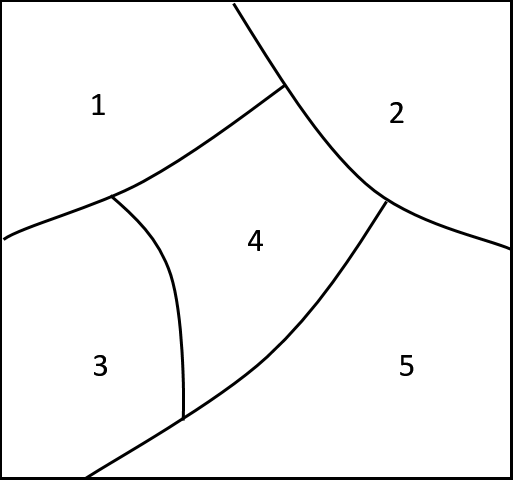
\includegraphics[width=3.8cm]{figures/初始分割结果.png}
    }
    \subfigure[对应的RAG]
    {
        \label{Fig.sub.2}
        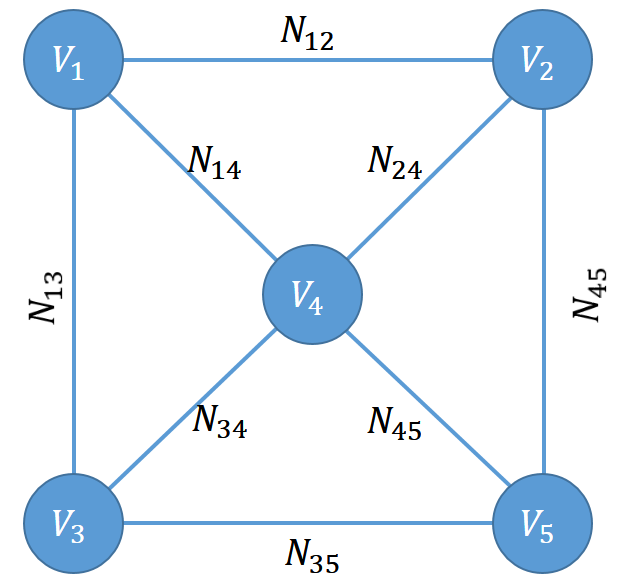
\includegraphics[width=3.8cm]{figures/对应的RAG.png}
    }
    \captionsetup{justification=centering}
    \caption{初始分割结果及其对应的RAG \\ Fig.\ref{初始分割结果及其对应的RAG} The Initial Segmentation Result and Its Corresponding RAG}
    \label{初始分割结果及其对应的RAG}
\end{figure}

使用RAG时,影响过分割图像合并结果的关键因素在于合并准则,主要有基于局部的合并准则和面向全局的合并准则两类。前者在局部范围内搜索满足合并条件的区域,并进行合并。后者从合并初始阶段开始,逐次合并全局最优的两个相邻区域,直到满足合并终止条件。面向全局的合并准则每次搜索全局最优的相邻区域进行合并,能及时针对每次合并产生的变化作出调整,精度较高,在合并准则确定的情况下,对于同一幅图像的合并过程相同,分割过程稳定性较好。合并准则中具体涵盖的特征多包括面积、均值、方差等初级视觉特征,而基于人体知觉的语义特征等高级特征较少应用于区域合并。

图\ref{RAG算法运算结果示意图}为RAG算法运算结果的示意图,图像中,黑色的边为SLIC算法分割出来的超像素块的边界,黄色的点为RAG中的图节点,绿色的边为RAG中图节点之间的边,不存在RAG边的地方表示图节点相似度较低,RAG算法将图节点之间的边擦除掉了。原始图像中,包括背景的底色共有5种颜色,经过RAG算法的处理,可以明显看出,不同颜色的超像素块之间的RAG边消失,相同颜色的超像素块之间的RAG边依旧存在。

\begin{figure}[H]
    \centering
    \subfigure[RAG原始图像]{
    \label{Fig.sub.1}
    
\includegraphics[width=3.8cm]{figures/RAG原始图像.jpg}}
    \subfigure[SLIC和RAG分割结果]{
    \label{Fig.sub.2}
    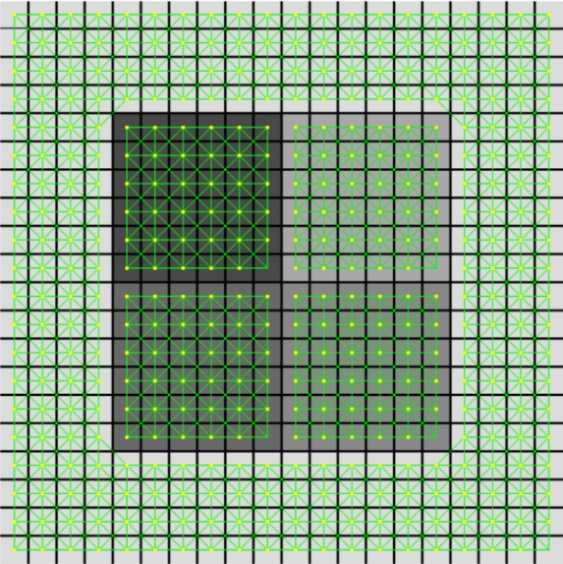
\includegraphics[width=3.8cm]{figures/SLIC算法和RAG算法分割结果.jpg}}
    \captionsetup{justification=centering}
    \caption{RAG算法运算结果示意图 \\ Fig.\ref{RAG算法运算结果示意图} RAG Algorithm Operation Result Diagram}
    \label{RAG算法运算结果示意图}
\end{figure}



\subsection{基于谱聚类和区域邻接图的最优分割算法}
基于谱聚类和区域邻接图的最优分割算法主要包括三个过程:SLIC算法进行图像过分割、谱聚类算法初次合并和区域邻接图进一步合并。下面依次介绍这三个过程。

(1) SLIC算法进行图像过分割

使用SLIC算法对输入原始图像进行过分割,在SLIC算法中,需要设定的参数有两个:超像素数量和紧密度参数。在本算法中,紧密度参数取值为常数$20$,超像素数量需要根据图像大小、景物大小、图像内容复杂度和算法应用场景进行设定,经过大量试验,对于Berkeley图像数据库(图像大小为$481\times321$)中的图像,兼顾算法运行时间,超像素数量设定为$500$即可。对于更大的图像,适当增加超像素数量能够提高算法分割质量。

(2) 谱聚类算法初步合并 

在使用 SLIC 算法对原始图像进行过分割生成超像素之后,首先进行超像素块的谱聚类过程。

对每一个超像素块,我们提取其$5$个特征构造相似度矩阵:包括$Lab$颜色空间超像素块的$l,a,b$颜色分量的均值,以及其等效位置$ x $坐标和$ y $坐标。

假设 SLIC 算法生成了$ N $个超像素块,则第$ i $个超像素块和第$ j $个超像素块间的距离将通过以下公式求得:
\[\begin{split}
D_{i,j}&=\sqrt{A_{i,j}+B_{i,j}} \\
A_{i,j}&=(l_i-l_j)^2+(a_i-a_j)^2+(b_i-b_j)^2 \\
B_{i,j}&=\frac{x_i-x_j}{SW}^2+\frac{y_i-y_j}{SW}^2
% D_{ij=√((l_i-l_j )^2+(a_i-a_j )^2+(b_i-b_j )^2+((x_i-x_j)/SW)^2+((y_i-y_j)/SW)^2 )
\end{split}\]

其中,$l,a,b$是超像素块在$Lab$颜色空间的颜色值,$x,y$是超像素块的等效位置。
$$
SW=\sqrt{((H\times W)/m)}
$$
$H$和$W$为图像的长度和宽度,$m$为一个常数,取值为$100$。

计算出距离矩阵$D$之后,对每一个超像素块,我们选择离它最近的$t$个超像素作为其邻居,则相似度矩阵$S$可以定义如下:
\begin{displaymath}
S_{i,j} = \left\{ \begin{array}{ll}

\exp{(\frac{-D^2_{i,j}}{2\sigma_i\sigma_j})}, & \textrm{超像素$i$和超像素$j$相邻}\\
0, & \textrm{其他}

\end{array} \right.
\end{displaymath}

其中,
$$
\sigma_i=\frac{1}{t}\sum_{k\in T}D_{i,k}
$$

超像素块$ k $属于超像素块$ i $的邻居超像素块的集合$T$。为了提高运行速度,将$t$取值为$5$。

得到相似度矩阵$S_{i,j}$之后,设定谱聚类算法的聚类数量,使用谱聚类算法进行聚类过程,实现超像素块的初步合并。

聚类数量的设定会影响谱聚类算法合并结果,如果聚类数量设定的不合理,会造成原始图像的欠分割,经过反复试验,针对,Berkeley图像数据库(图像大小为$481\times321$)和真实无人机航拍图像(图像大小为$1000\times1000$)而言,谱聚类数量设定为$30$时,谱聚类合并结果较为理想,当图像大小更大、内容较为复杂时,增加聚类数量能够得到更好的结果。

(3) 区域邻接图进一步合并

谱聚类算法对过分割图像的合并过程中,主要的合并依据为相似度矩阵$S$。在构造相似度矩阵$S$的过程中,超像素块之间的相似度主要通过公式进行计算,上式中,主要考虑了某一个超像素块在全局范围内与哪一个超像素块最相似,进而依据全局范围内的相似性进行聚类合并。RAG则将区域合并的重点放在衡量某一个超像素块与周围超像素块的相似性上。也就是说谱聚类算法的合并过程是一种面向全局的区域合并过程,而RAG的合并过程则是一种面向局部的区域合并过程,两种算法配合使用,能够兼顾全局和局部超像素块的相似性度量和合并。

在对谱聚类算法合并结果进行RAG区域合并的过程中,主要的参数为区域相似度阈值。当两个区域的相似度小于阈值时,合并这两个区域,反之不进行合并。区域相似度阈值$threshold$通过自适应的方式进行设定,以下对自适应方法进行介绍。

定义阈值$threshold$为变量$T$。同时,定义变量$MaxEdges$,其定义为在$Lab$颜色空间中,超像素块$k$与相邻超像素块集合$L$的最大颜色距离,$l\in L$时,颜色距离定义为:
$$
E_{k,l}=\sqrt{(l_i-l_j)^2+(a_i-a_j)^2+(b_i-b_j)^2}
$$

则$MaxEdges$定义为:
$$
MaxEdges=\max{(E_{k,l}),l\in L}
$$

$MaxEdges$求出来之后,可以求得$T$
$$
T=mean{(MaxEdges)}-\frac{std(MaxEdges)}{2}
$$

$mean(MaxEdges)$为$MaxEdges$的均值,$std(MaxEdges)$为$MaxEdges$ 的标准差。

为了避免阈值$T$过小影响合并过程,重新定义$T$如下:

\begin{displaymath}
T' = \left\{ \begin{array}{ll}

T, & \textrm{if $T>10$}\\
10, & \textrm{otherwise}

\end{array} \right.
\end{displaymath}

